\subsection{Overview}
\begin{frame}
    \frametitle{The Man}
    \begin{center}
        
\includegraphics[scale=.5]{images/paimei/pstalker_demo.jpg} \\
    \end{center}
\end{frame}

\begin{frame}[t]
    \frametitle{What is it?}
    \begin{itemize}
        \item It's a win32 reverse engineering framework
        \item Written entirely in Python
        \item Think of PaiMei as an RE swiss army knife
        \item Already proven effective for a number of tasks
            \pedbullet{Fuzzer assistance}
            \pedbullet{Code coverage tracking}
            \pedbullet{Data flow tracking}
            \pedbullet{A beta tester used it to solve the T2'06 RE challenge}
    \end{itemize}
    \begin{block}{My hopes and dreams}
    That with community support and contributions, PaiMei can do for RE dev what Metasploit does for exploit dev
    \end{block}
\end{frame}

\begin{frame}[t]
    \frametitle{Motivation: Rapid Development}
    \begin{itemize}
        \item Avoid the learning / re-learning curve of various SDKs
        \item Develop in a higher level language
            \pedbullet{Easy management of arbitrary data structures}
            \pedbullet{Less code}
            \pedbullet{Less debugging of the actual tool}
        \item Build data representation \alert{into} the framework, as opposed to an after-thought
            \pedbullet{Of course, coming from Pedram, this translates into graphing}
    \end{itemize}
\end{frame}

\begin{frame}[t]
    \frametitle{Motivation: Homogenous Environment}
    \begin{itemize}
        \item Making tools and languages talk to one another is tedious
            \pedbullet{IDA vs. OllyDbg vs. MySQL}
            \pedbullet{C/C++ vs. Python}
        \item Centralized tool creation vs. the old school:
            \pedbullet{Launch debugger}
            \pedbullet{Run plug-in}
            \pedbullet{Save output to disk}
            \pedbullet{Parse output through Perl into IDC}
            \pedbullet{Import into IDA}
    \end{itemize}
\end{frame}

\begin{frame}[t]
    \frametitle{Core Components}
    \begin{block}{PyDbg}
        A pure Python win32 debugger abstraction class
    \end{block}
    \begin{block}{pGRAPH}
        An abstraction library for representing graphs as a collection of nodes, edges and clusters
    \end{block}
    \begin{block}{PIDA}
        A binary abstraction library, built on top of pGRAPH, for representing binaries as a collection of functions, basic blocks and instructions
    \end{block}
\end{frame}

\begin{frame}[t]
    \frametitle{Extended Components}
    \begin{block}{Utilities}
        A set of abstraction classes for accomplishing various repetitive tasks
    \end{block}
    \begin{block}{Console}
        A pluggable WxPython GUI for quickly and efficiently rolling out your own sexy RE tools
    \end{block}
    \begin{block}{Scripts}
        Individual scripts built on the framework
    \end{block}
\end{frame}

\begin{frame}[t]
    \frametitle{PyDbg}
    Exposes all the expected functionality and then some ...
    \begin{columns}[T]
        \column{.6\textwidth}
            \begin{itemize}
                \item \alert<2>{Process, module, and thread enumeration}
                    \mode<article>{\pedbullet{enumerate\_processes(), enumerate\_modules(), enumerate\_threads(), attach(), load(), suspend\_thread(), resume\_thread()}}
                \item \alert<3>{Hardware, software and memory breakpoints}
                    \mode<article>{\pedbullet{bp\_set\_hw(), bp\_set(), bp\_set\_mem(), bp\_del\_hw(), bp\_del(), bp\_del\_mem(), bp\_is\_ours\_mem()}}
                \item \alert<4>{Memory read/write/alloc and smart dereferencing}
                    \mode<article>{\pedbullet{read(), write(), virtual\_alloc(), virtual\_query(), smart\_dereference()}}
                \item \alert<5>{Memory snapshots and restores}
                    \mode<article>{\pedbullet{process\_snapshot(), process\_restore()}}
                \item \alert<6>{Stack and SEH unwinding}
                    \mode<article>{\pedbullet{stack\_unwind(), seh\_unwind()}}
                \item \alert<7>{Exception and event handling}
                    \mode<article>{\pedbullet{set\_callback()}}
                \item \alert<8>{Disassembly (libdasm)}
                    \mode<article>{\pedbullet{disasm(), disasm\_around()}}
                \item \alert<9>{Utility functions}
                    \mode<article>{\pedbullet{flip\_endian(), flip\_endian\_dword(), func\_resolve(), hex\_dump(), to\_binary(), to\_decimal()}}
            \end{itemize}
        \column{.4\textwidth}
            \mode<presentation>{\only<2->{
            \begin{block}{Example API}
                \texttt{
                    \only<2>{\\ enumerate\_processes() \\ enumerate\_modules() \\ enumerate\_threads() \\ attach() \\ load() \\ suspend\_thread() \\ resume\_thread()}
                    \only<3>{\\ bp\_set\_hw() \\ bp\_set() \\ bp\_set\_mem() \\ bp\_del\_hw() \\ bp\_del() \\ bp\_del\_mem() \\ bp\_is\_ours\_mem()}
                    \only<4>{\\ read() \\ write() \\ virtual\_alloc() \\ virtual\_query() \\ smart\_dereference()}
                    \only<5>{\\ process\_snapshot() \\ process\_restore()}
                    \only<6>{\\ stack\_unwind() \\ seh\_unwind()}
                    \only<7>{\\ set\_callback()}
                    \only<8>{\\ disasm() \\ disasm\_around()}
                    \only<9>{\\ flip\_endian() \\ flip\_endian\_dword() \\ func\_resolve() \\ hex\_dump() \\ to\_binary() \\ to\_decimal()}
                }
            \end{block}
            }}
    \end{columns}
\end{frame}

\begin{frame}[t, fragile]
    \frametitle{PyDbg: Example}
    \begin{block}{Abstracted interface allows for painless development}
    \begin{tiny}
    \begin{semiverbatim}
        from \alert{pydbg} import *
        from \alert{pydbg.defines} import *
        
        def \alert{handler_breakpoint} (pydbg):
            \emph{# ignore the first windows driven breakpoint.}
            if \alert{pydbg.first_breakpoint}:
                return DBG_CONTINUE
        
            print "ws2_32.recv() called from thread \%d @\%08x" \% \\
                \alert{pydbg.dbg.dwThreadId},
                \alert{pydbg.exception_address})
        
            return DBG_CONTINUE
        
        \alert{dbg = pydbg()}
        
        \emph{# register a breakpoint handler function.}
        \alert{dbg.set_callback}(EXCEPTION_BREAKPOINT, handler_breakpoint)
        \alert{dbg.attach}(XXXXX)
        
        recv = \alert{dbg.func_resolve}("ws2_32", "recv")
        \alert{dbg.bp_set}(recv)
        
        \alert{pydbg.run}()
    \end{semiverbatim}
    \end{tiny}
    \end{block}
\end{frame}

\begin{frame}[t]
    \frametitle{PyDbg: Random Idea Implementation}
    \begin{block}{The problem}
        I want to solve the F-Secure T2'06 challenge ... but I'm lazy.
    \end{block}
    \begin{enumerate}
        \item Open the binary in IDA
        \item Locate password read and process exit
        \item Set breakpoints on both
        \item The first time a password is read, snapshot
        \item When the exit is reached, restore
        \item Read the buffer address off the stack
        \item Change the password
        \item Continue
    \end{enumerate}
\end{frame}

\begin{frame}[t]
    \frametitle{pGRAPH}
    Exposes much of the expected functionality:
    \begin{columns}[T]
        \column{.6\textwidth}
            \begin{itemize}
                \item \alert<2>{Node and edge management}
                    \mode<article>{\pedbullet{add\_node(), add\_edge(), del\_node(), del\_edge()}}
                \item \alert<3>{Node and edge searching}
                    \mode<article>{\pedbullet{find\_node(), find\_edge(), edges\_from(), edges\_to()}}
                \item \alert<4>{Graph manipulation}
                    \mode<article>{\pedbullet{graph\_cat(), graph\_sub(), graph\_up(), graph\_down(), graph\_intersect(), graph\_proximity()}}
                \item \alert<5>{Graph rendering}
                    \mode<article>{\pedbullet{render\_graph\_graphviz(), render\_graph\_gml(), render\_graph\_udraw()}}
            \end{itemize}
            \only<6>{Why do we need this library?}
        \column{.4\textwidth}
            \mode<presentation>{\only<2-5>{
            \begin{block}{Example API}
                \texttt{
                    \only<2>{\\ add\_node() \\ add\_edge() \\ del\_node() \\ del\_edge()}
                    \only<3>{\\ find\_node() \\ find\_edge() \\ edges\_from() \\ edges\_to()}
                    \only<4>{\\ graph\_cat() \\ graph\_sub() \\ graph\_up() \\ graph\_down() \\ graph\_intersect() \\ graph\_proximity()}
                    \only<5>{\\ render\_graph\_graphviz() \\ render\_graph\_gml() \\ render\_graph\_udraw()}
                }
            \end{block}
            }}
    \end{columns}
\end{frame}

\begin{frame}[t]
    \frametitle{PIDA}
    \begin{itemize}
        \item Extends from pGRAPH to represent binaries as a \alert{graph of graphs}
        \item PIDA databases are propogated by an IDA Python script \alert{pida\_dump.py}
            \pedbullet{This is important, I will show it to you in a second}
        \item The database is serialized to a zlib compressed \alert{.pida} database
        \item PIDA enumerates basic blocks and discovers RPC routines
        \item The .pida database can later be loaded independent of IDA
        \item All the aforementioned graph functionality is available for (ab)use
        \item \alert{Quick demo}
    \end{itemize}
\end{frame}

\begin{frame}[t, fragile]
    \frametitle{PIDA: Contrived Example}
    \begin{block}{Again, abstracted interface allows for painless development}
    \begin{tiny}
    \begin{semiverbatim}
        import \alert{pida} import *
        
        module = \alert{pida.load}("some\_file.pida")
        
        \emph{# render a function graph in uDraw format for the entire module.}
        fh = open("graphs/functions.udg", "w+")
        fh.write(module.\alert{render\_graph\_udraw()})
        fh.close()
        
        \emph{# step through each function in the module:}
        for function in module.\alert{functions}.values():
            \emph{# if we found the function we are interested in:}
            if function.\alert{name} == "some\_function":
                \emph{# step through each basic block in the function.}
                for bb in function.\alert{basic\_blocks}.values():
                    print "\\t\%08x - \%08x" \% (bb.ea\_start, bb.ea\_end)
                    \emph{# print each instruction in each basic block.}
                    for ins in bb.\alert{instructions}.values():
                        print "\\t\\t\%s" \% ins.\alert{disasm}
        
                \emph{# render a GML graph of this function.}
                fh = open("graphs/function.gml", "w+")
                fh.write(function.\alert{render\_graph\_gml()})
                fh.close()
    \end{semiverbatim}
    \end{tiny}
    \end{block}
\end{frame}

\begin{frame}[t, fragile]
    \frametitle{PIDA: Contrived Example}
    \begin{block}{...Continued}
    \begin{tiny}
    \begin{semiverbatim}
            \emph{# if we found the second function we are interested in.}
            if function.\alert{ea\_start} == 0xdeadbeef:
                
                \emph{# render a uDraw format proximity graph.}
                fh = open("graphs/proximity.udg", "w+")
                
                \emph{# look 3 levels up and 2 levels down.}
                prox\_graph = module.\alert{graph\_proximity}(function.id, 3, 2)
                fh.write(prox\_graph.\alert{render\_graph\_udraw}())
                fh.close()
    \end{semiverbatim}
    \end{tiny}
    \end{block}
    Together, PIDA and PyDbg offer a powerful combination for building a variety of tools. Consider for example the ease of re-creating Process Stalker on top of this platform.
\end{frame}

\begin{frame}[t, fragile]
    \frametitle{PIDA: Real World Example}
    \begin{block}{}
        Locate all functions within a binary that open a file and display the execution path from the entry point to the call of interest...
    \end{block}
    \begin{block}{}
    \begin{tiny}
    \begin{semiverbatim}
\emph{\textcolor{blue}{# for each function in the module}}
for function in module.functions.values():
    \emph{\textcolor{blue}{# create a downgraph from the current routine and locate the calls to [Open|Create]File[A|W]}}
    downgraph = module.graph\_down(function.ea\_start, -1)
    matches   = [node for node in downgraph.nodes.values() if re.match(".*(create|open)file.*", \\
                node.name, re.I)]
    upgraph   = pgraph.graph()

    \emph{\textcolor{blue}{# for each matching node create a temporary upgraph and add it to the parent upgraph.}}
    for node in matches:
        tmp\_graph = module.graph\_up(node.ea\_start, -1)
        upgraph.graph\_cat(tmp\_graph)

    \emph{\textcolor{blue}{# write the intersection of the down graph from the current function and the upgraph from}}
    \emph{\textcolor{blue}{# the discovered interested nodes to disk in gml format.}}
    downgraph.graph\_intersect(upgraph)

    if len(downgraph.nodes):
        fh = open("%s.gml" % function.name, "w+")
        fh.write(downgraph.render\_graph\_gml())
        fh.close()
    \end{semiverbatim}
    \end{tiny}
    \end{block}
    Together, PIDA and PyDbg offer a powerful combination for building a variety of tools. Consider for example the ease of re-creating Process Stalker on top of this platform.
\end{frame}

\begin{frame}[t]
    \frametitle{Utilities}
    \begin{itemize}
        \item Classes for further abstracting frequently repeated functionality:
            \pedbullet{Code Coverage}
            \pedbullet{Crash Binning}
            \pedbullet{Process Stalker}
            \pedbullet{uDraw Connector}
    \end{itemize}
\end{frame}

\begin{frame}[t]
    \frametitle{Utility: Code Coverage}
    \begin{itemize}
        \item Simple container for storing code coverage data
        \item Supports persistant storage to MySQL or serialized file
        \item You can use this class to keep track of where you have been
        \item Examples:
            \pedbullet{Process Stalker}
            \pedbullet{Individual fuzzer test case tracking}
    \end{itemize}
\end{frame}

\begin{frame}[t]
    \frametitle{Utility: Crash Binning}
    \begin{itemize}
        \item Simple container for categorizing and storing "crashes"
        \item Stored crashes are organized in bins by exception address
        \item The in-house version of this class goes one step further by categorizing on path as well (stack unwind)
        \item The \texttt{crash\_synopsis()} routine generates detailed crash reports:
            \pedbullet{Exception address, type and violation address}
            \pedbullet{Offending thread ID and context}
            \pedbullet{Disassembly around the exception address}
            \pedbullet{Stack and SEH unwind information}
        \item This class is extremely useful for fuzzer monitoring
            \pedbullet{\emph{ex:} 250 crashes vs. 248 crashes at \alert{x} and 2 crashes at \alert{y}}
       \item \emph{Note to Pedram}: Mention the Excel file format exploit "fuzzer"
    \end{itemize}
\end{frame}

\begin{frame}[t]
    \frametitle{Utility: Process Stalker}
    \begin{itemize}
        \item Abstracted interface to Process Stalking style code coverage
        \item Currently only being used by the pstalker GUI module
        \item A command line interface can be easily built
        \item The class handles all the basics:
            \pedbullet{Re-basing and setting breakpoints in the main module}
            \pedbullet{Re-basing and setting breakpoints in loaded libraries}
            \pedbullet{Recording, with or without context data, hit breakpoints}
            \pedbullet{Monitoring for access violations}
            \pedbullet{Exporting (through the code coverage class) to MySQL}
    \end{itemize}
\end{frame}

\begin{frame}[t]
    \frametitle{Utility: uDraw(Graph) Connector}
    Python interface to the uDraw(Graph) API. Much of the uDraw API currently remains unwrapped. \emph{Note to Pedram}: Mention how badass uDraw is.
    \begin{columns}[T]
        \column{.6\textwidth}
            \begin{itemize}
                \item \alert<2>{Draw graphs}
                    \mode<article>{\pedbullet{graph\_new(), graph\_update()}}
                \item \alert<3>{Move the graph}
                    \mode<article>{\pedbullet{focus\_node(), layout\_improve\_all(), scale(), open\_survey\_view()}}
                \item \alert<4>{Modify the graph}
                    \mode<article>{\pedbullet{change\_element\_color(), window\_background(), window\_status(), window\_title()}}
                \item \alert<5>{Register callbacks}
                    \mode<article>{\pedbullet{set\_command\_handler()}}
            \end{itemize}
        \column{.4\textwidth}
            \mode<presentation>{\only<2->{
            \begin{block}{Example API}
                \texttt{
                    \only<2>{\\ graph\_new() \\ graph\_update()}
                    \only<3>{\\ focus\_node() \\ layout\_improve\_all() \\ scale() \\ open\_survey\_view()}
                    \only<4>{\\ change\_element\_color() \\ window\_background() \\ window\_status() \\ window\_title()}
                    \only<5>{\\ set\_command\_handler()}
                }
            \end{block}
            }}
    \end{columns}
\end{frame}

\begin{frame}
    \frametitle{How it All Ties Together}
    \begin{center}
        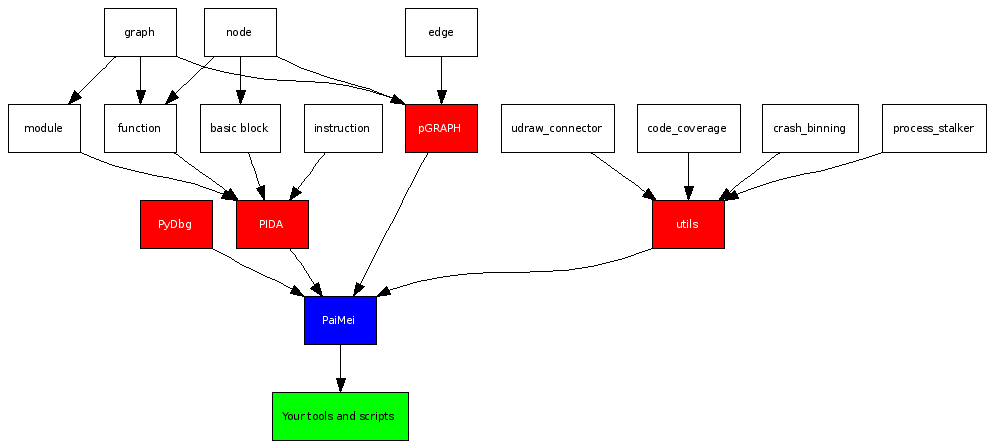
\includegraphics[scale=.33]{images/paimei/paimei_relationship_graph.png} \\
    \end{center}
\end{frame}

\begin{frame}
    \frametitle{GUI Overview}
    \begin{itemize}
        \item Some complex tools are not suitable for the command line
        \item The PaiMei console provides a base for new GUI modules
        \item Development for the framework is well documented (I think)
        \item Allows you to focus your efforts on the tool
        \item GUI modules follow the naming convention PAIMEIxxxx
    \end{itemize}
\end{frame}

\begin{frame}
    \frametitle{GUI General layout}
    \begin{itemize}
        \item Modules are independent of one another
            \pedbullet{Though you can push / pull data between them}
        \item Each module represented by a notebook icon
        \item Entire right pane is controlled by the module
        \item Left status bar displays console wide messages
        \item Right status bar is owned by the current module
        \item \emph{Connections} menu establishes connectivity to MySQL and uDraw
        \item \emph{Advanced} menu exposes log window clearing and CLI
        \item The CLI (Command Line Interface) is a full Python interpreter and allows you to interact with any portion of the console.
            \pedbullet{Explicitly documented module member variables are listed on the right-hand side of the CLI}
    \end{itemize}
\end{frame}


\subsection{Command Line Tools}
\begin{frame}[t]
    \frametitle{DPC: Debuggee Procedure Call}
    Allows you to call arbitrary functions in your target. Implemented using a simple process:
    \begin{columns}[T]
        \column{.5\textwidth}
            \uncover<2->{
                \begin{enumerate}
                    \item \uncover<2->{Allocate space for new instructions}
                    \item \uncover<3->{Reverse the argument list}
                    \item \uncover<4->{\texttt{PUSH} numeric arguments directly}
                    \item \uncover<5->{Allocate space for string arguments and \texttt{PUSH} address}
                    \item \uncover<6->{Write the \texttt{CALL} instruction}
                    \item \uncover<7->{Write an \texttt{INT 3} to regain control}
                \end{enumerate}
            }
        \column{.5\textwidth}
            \alert{\texttt{procedure("pedram", 26)}}
            \uncover<2->{
                \begin{block}{}\texttt{                                 \\
                    \uncover<4->{PUSH 26}                               \\
                    \uncover<5->{PUSH \textcolor{orange}{0x12345678}}   \\
                    \uncover<6->{CALL procedure}                        \\
                    \uncover<7->{INT 3}
                }\end{block}
                \uncover<5->{
                    \begin{block}{}
                        \textcolor{orange}{\texttt{0x12345678:}} \emph{"pedram"}
                    \end{block}
                }
            }
    \end{columns}
\end{frame}

\begin{frame}[t]
    \frametitle{DPC: Usage}
    \begin{itemize}
        \item Once attached you are given a command prompt
        \item Any Python statement is valid
        \item \texttt{dbg} references current PyDbg instance
        \item Convenience wrappers exist for memory manipulaton
            \pedbullet{\texttt{alloc(), free(), free\_all(), show\_all()}}
        \item Assigned variables are not persistant!
            \pedbullet{Use \texttt{glob} for that}
            \pedbullet{\texttt{print glob} to display what you have assigned}
        \item \texttt{dpc(procedure, *args, **kwargs)}
            \pedbullet{kwargs are for fast call support}
        \item Took me less than 30 minutes to write the 1st version of this tool
    \end{itemize}
\end{frame}

\begin{frame}[t]
    \frametitle{DPC: Example One}
    \begin{columns}
        \column{.5\textwidth}
            \begin{block}{Taking shortcuts}
                \begin{itemize}
                    \item The following routine would have taken a good effort to reverse
                    \item Using DPC however the functionality is quickly evident
                    \item Call out the answer if you know it
                \end{itemize}
            \end{block}
        \column{.5\textwidth}
            \begin{center}
            \begin{tabular}{|l|r|r|}                                                                               \hline
                \cellcolor{lightblue}Input Range & \cellcolor{lightblue}Return & \cellcolor{lightblue} $\Delta$ \\ \hline
                \uncover <2->{25-29 & \only <2>{\cellcolor{orange}}29 & 6}                                      \\ \hline
                \uncover <3->{30-31 & \only <3>{\cellcolor{orange}}31 & 2}                                      \\ \hline
                \uncover <4->{32-37 & \only <4>{\cellcolor{orange}}37 & 6}                                      \\ \hline
                \uncover <5->{38-41 & \only <5>{\cellcolor{orange}}41 & 4}                                      \\ \hline
                \uncover <6->{42-43 & \only <6>{\cellcolor{orange}}43 & 2}                                      \\ \hline
                \uncover <7->{44-47 & \only <7>{\cellcolor{orange}}47 & 4}                                      \\ \hline
                \uncover <8->{48-53 & \only <8>{\cellcolor{orange}}53 & 6}                                      \\ \hline
                \uncover <9->{54-59 & \only <9>{\cellcolor{orange}}59 & 6}                                      \\ \hline
                \uncover<10->{60-61 & \only<10>{\cellcolor{orange}}61 & 2}                                      \\ \hline
                \uncover<11->{62-67 & \only<11>{\cellcolor{orange}}67 & 6}                                      \\ \hline
                \uncover<12->{68-71 & \only<12>{\cellcolor{orange}}71 & 4}                                      \\ \hline
            \end{tabular}
            \end{center}
    \end{columns}
\end{frame}

\begin{frame}[t]
    \frametitle{DPC: Example Two}
        Here's another one...
        \begin{center}
        \begin{tabular}{|l|l|r|r|}                                                                                                  \hline
            \cellcolor{lightblue}Arg 1 & \cellcolor{lightblue}Arg 2 & \cellcolor{lightblue} Arg 3 & \cellcolor{lightblue} Return \\ \hline
            \uncover <2->{paimei & eyebrow & 25    & \only <2>{\cellcolor{orange}}0x00000001}                                    \\ \hline
            \uncover <3->{paimei & apple   & 50    & \only <3>{\cellcolor{orange}}0x00000001}                                    \\ \hline
            \uncover <4->{paimei & pear    & 69    & \only <4>{\cellcolor{orange}}0xFFFFFFFF}                                    \\ \hline
            \uncover <5->{pai    & paimei  & 666   & \only <5>{\cellcolor{orange}}0xFFFFFFFF}                                    \\ \hline
            \uncover <6->{paimei & paimei  & 31337 & \only <6>{\cellcolor{orange}}0x00000000}                                    \\ \hline
            \uncover <7->{pai    & paimei  & 3     & \only <7>{\cellcolor{orange}}0x00000000}                                    \\ \hline
        \end{tabular}
        \end{center}
\end{frame}

\begin{frame}
    \frametitle{DPC: (Quick) Live Demo}
    \begin{center}
        
\includegraphics[scale=.5]{images/paimei/dpc_demo.jpg} \\
    \end{center}
\end{frame}

\begin{frame}[t]
    \frametitle{OllyDbg Connector}
    \begin{itemize}
        \item PyDbg is designed for mostly non-interactive functionality
        \item This two-part tool adds live graphing functionality to OllyDbg
        \item Part 1: Receiver
            \pedbullet{Socket server for OllyDbg}
            \pedbullet{Receives module name, base address and offset from plug-in}
            \pedbullet{Socket client to uDraw(Graph)}
            \pedbullet{Loads specified PIDA database and generates graph}
        \item Part 2: Connector
            \pedbullet{Registers hotkeys for transmitting location to receiver}
            \pedbullet{\alert{,} Step into and xmit current location}
            \pedbullet{\alert{.} Step over and xmit current location}
            \pedbullet{\alert{/} Xmit current location}
    \end{itemize}
\end{frame}

\begin{frame}
    \frametitle{OllyDbg Connector: Live Demo}
    \begin{center}
        
\includegraphics[scale=.25]{images/paimei/ollydbg_connector_demo.jpg} \\
    \end{center}
\end{frame}

\begin{frame}[t]
    \frametitle{Stack Integrity Monitor}
    \begin{itemize}
        \item Tracking down the source of a complete stack smash is tedious
        \item I had to do a bunch one day so I wrote a 150 line PyDbg script
        \item How it works:
            \pedbullet{Instantiate a debugger object and attach to the target program}
            \pedbullet{Set a breakpoint where we want the trace to start, this can be as simple as setting a break on recv()}
            \pedbullet{Once the breakpoint is hit, set the active thread to single step}
            \pedbullet{When a CALL instruction is reached, copy the stack and return addresses to an internal "mirror" list}
            \pedbullet{When a RET instruction is reached, walk through the "mirror" list and verify that the values match the actual stack}
            \pedbullet{When the last saved return address is reached, pop it off the internal "mirror" list}
    \end{itemize}
\end{frame}

\begin{frame}[t, fragile]
    \frametitle{Stack Integrity Monitor: Before}
    \begin{tiny}
    \begin{semiverbatim}
[INVALID]:41414141 Unable to disassemble at 41414141 from thread 568 caused
          access violation when attempting to read from 0x41414141

CONTEXT DUMP
  EIP: 41414141 Unable to disassemble at 41414141
  EAX: 00000001 (         1) -> N/A
  EBX: 0259eedc (  39448284) -> AAAAAAAAAAAAAA....AAAAAAAAAAAAAAAAAA (stack)
  ECX: 00000000 (         0) -> N/A
  EDX: ffffffff (4294967295) -> N/A
  EDI: 00000000 (         0) -> N/A
  ESI: 0259f102 (  39448834) -> AAAAAAAAAAAAAA....AAAAAAAAAAAAAAAAAA (stack)
  EBP: 00000001 (         1) -> N/A
  ESP: 0259e2d4 (  39445204) -> AAAAAAAAAAAAAA....AAAAAAAAAAAAAAAAAA (stack)
  +00: 41414141 (1094795585) -> N/A
  +04: 41414141 (1094795585) -> N/A
  +08: 41414141 (1094795585) -> N/A
  +0c: 41414141 (1094795585) -> N/A
  +10: 41414141 (1094795585) -> N/A
  +14: 41414141 (1094795585) -> N/A

disasm around:
        0x41414141 Unable to disassemble
    \end{semiverbatim}
    \end{tiny}
\end{frame}

\begin{frame}[t, fragile]
    \frametitle{Stack Integrity Monitor: After}
    \begin{tiny}
    \begin{semiverbatim}
    0259fc24: TmRpcSrv.dll.65741721
    0259e7b4: StRpcSrv.dll.65671190
    0259e7a8: Eng50.dll.61181d8c
    0259e790: Eng50.dll.611819a0
    0259e564: Eng50.dll.61181a50
    0259e2d0: Eng50.dll.61190fa4 --> 41414141
    0259e03c: Eng50.dll.61190fd2
    
    STACK INTEGRITY VIOLATON AT: Eng50.dll.61194b8e
    analysis took 35 seconds
    \end{semiverbatim}
    \end{tiny}
    Examining the vicinity of the last return address in the list, we find:
    \begin{tiny}
    \begin{semiverbatim}
    61190FC7 lea edx, [esp+288h+szShortPath]
    61190FCB push esi
    61190FCC push edx
    \alert{61190FCD call _wcscpy }
    61190FD2 add esp, 8
    \end{semiverbatim}
    \end{tiny}
\end{frame}

\begin{frame}[t]
    \frametitle{Proc Peek}
    \begin{itemize}
        \item This two-part tool was designed for discovering \emph{low hanging fruit} vulnerabilities
            \pedbullet{Which, believe it or not, is quite effective}
        \item The first half of the tool is a static reconnaissance phase
            \pedbullet{\emph{proc\_peek\_recon.py}}
        \item The second half of the tool is a run-time analysis phase
            \pedbullet{\emph{proc\_peek.py} and \emph{PAIMEIpeek}}
    \end{itemize}
    \begin{block}{General philosophy}
        With minimal effort, generate a list of locations that can be easily monitored and \emph{checked off}. This approach is great for 1st phase auditing and can be handed off to an intern.
    \end{block}
\end{frame}

\begin{frame}[t]
    \frametitle{Proc Peek: proc\_peek\_recon.py}
    \begin{itemize}
        \item IDA Python script
        \item Looks for \emph{interesting} locations, or \alert{peek points}
            \begin{itemize}
                \item Inline \texttt{memcpy()} and \texttt{strcpy() routines}
                \item Calls to API that accept format string tokens
                    \pedbullet{Ignoring ones that do not contain \texttt{\%s}}
                \item Calls to potentially \emph{dangerous} API such as \texttt{strcat()}, \texttt{strcpy()}, etc...
            \end{itemize}
        \item Discovered peek points are written to a file or database
    \end{itemize}
\end{frame}

\begin{frame}[t]
    \frametitle{Proc Peek: proc\_peek.py}
    \begin{itemize}
        \item PyDbg based script (a bit dated)
        \item Attach to the target process
        \item Set breakpoints on each peek point
        \item When a breakpoint is hit:
            \pedbullet{Present the user with relevant information}
            \pedbullet{Prompt for action: \emph{ignore}, \emph{continue}, \emph{make notes}}
        \item Supports automated keyword searching (Hoglund: \emph{Boron tagging})
        \item Also features Winsock recv() tracking
    \end{itemize}
\end{frame}


\subsection{GUI and Tools}
\begin{frame}[t]
    \frametitle{Proc Peek: PAIMEIpeek}
    \begin{itemize}
        \item Also PyDbg based, the GUI version of the last script
        \item Less of an interactive tool, more of a data sampling utility
        \item Again, set breakpoints on each peek point
        \item When a breakpoint is hit:
            \pedbullet{Record the time and contextual information to the database}
            \pedbullet{Search the context for user-specified keywords}
    \end{itemize}
\end{frame}

\begin{frame}
    \frametitle{PAIMEIpeek: Demo}
    \begin{center}
        
\includegraphics[scale=.5]{images/paimei/peek_demo.png} \\
    \end{center}
\end{frame}

\begin{frame}[t]
    \frametitle{PAIMEIdocs}
    \begin{itemize}
        \item HTML documentation browser
        \item Use the control bar at the top to load general or developer specific documentation
        \item Not all that exciting
    \end{itemize}
\end{frame}

\begin{frame}[t]
    \frametitle{PAIMEIexplore}
    \begin{itemize}
        \item The \emph{hello world} of the console
        \item The in-house version has a bit more functionality
        \item To use:
            \pedbullet{Load a PIDA database}
            \pedbullet{Double click the PIDA database}
            \pedbullet{Browse through the explorer tree}
            \pedbullet{Select a function to display disassembly}
            \pedbullet{Connect to uDraw}
            \pedbullet{Graph a function through the right-click context menu}
    \end{itemize}
\end{frame}

\begin{frame}[t]
    \frametitle{PAIMEIfilefuzz}
    \begin{itemize}
        \item File fuzzing and exception monitoring tool built on PaiMei
        \item Developed by Cody Pierce
        \item Loads a target file
        \item Generates mutations based at specified offset / range, variable length and byte values
            \pedbullet{More advanced features include, additive mutations}
        \item Supports mid-session pause and resume
        \item Features predictable completion time and run-time statistics
        \item In-house experimental features:
            \pedbullet{Auto file discovery}
            \pedbullet{Auto handler discovery}
            \pedbullet{Auto fuzz}
            \pedbullet{ie: Give it a laptop and go}
    \end{itemize}
\end{frame}

\begin{frame}[t]
    \frametitle{PAIMEIdiff}
    \begin{itemize}
        \item A binary diffing tool built on PaiMei
        \item Being developed by Peter Silberman
        \item Still an early beta and not currently distributed
        \item Heuristic based diffing engine (like Zynamics BinDiff)
        \item The goal of the module is to allow the user to deeply control the diffing algorithm
        \item Customized algorithms can be saved for later use
        \item This will likely lead to job specific sets:
            \pedbullet{Malware analysis}
            \pedbullet{Generic patch diffing}
            \pedbullet{Microsoft patch diffing}
            \pedbullet{Etc...}
    \end{itemize}
\end{frame}

\begin{frame}[t]
    \frametitle{PAIMEIdiff: Supported Heuristics}
    Some of these were gleaned from the Zynamics Security white papers:
    \begin{itemize}
        \item API calls
        \item Argument and variable sizes
        \item Constants
        \item Control flow
        \item CRC
        \item Name
        \item NECI (graph heuristics)
        \item Recursive calls
        \item Size
        \item Small Prime Product (SPP)
        \item "Smart" MD5
        \item Stack frame
        \item String references
    \end{itemize}
\end{frame}

\begin{frame}[t]
    \frametitle{PAIMEIpstalker}
    \begin{itemize}
        \item Code coverage recording tool
        \item This is the "next generation" of Process Stalker
        \item All metadata is stored to MySQL
        \item Three step approach:
            \pedbullet{Setup data sources}
            \pedbullet{Capture code coverage data}
            \pedbullet{Explore captured data}
        \item Filtering support allows you to pinpoint interesting code locations
    \end{itemize}
\end{frame}


\subsection{Exercises}
\begin{frame}
    \frametitle{Basic Exercises}
    \begin{itemize}
        \item Write a PIDA script to locate utility functions
        \item Use DPC to decipher one of the located utility functions
        \item Write a PIDA script to find all paths to a specific API
        \item Write a PyDbg script to sample data crossing a specific point
        \item For a more in-depth project, see the next two slides
    \end{itemize}
\end{frame}

\begin{frame}
    \frametitle{Malware Profiler}
    \begin{itemize}
        \item I will never get around to this, so someone else do it
        \item Post unpacking / PIDA conversion, static analysis tool
        \item Step through the call chains within the binary
            \pedbullet{Mark common sequences with a high level label}
            \pedbullet{Automatically extract information such as mutex name, startup keys, etc..}
        \item Can help narrow analysis areas, ie:
            \pedbullet{Glean what you can through live analysis}
            \pedbullet{Automatically tag and command statically recognized code sequences}
            \pedbullet{What you are left with will be the more interesting sections}
        \item The tool should be driven by XML configuration files (next slide)
    \end{itemize}
\end{frame}

\begin{frame}[fragile]
    \frametitle{Malware Profiler: Continued}
    \begin{block}{Theorized example XML}
    \begin{tiny}
    \begin{semiverbatim}
        <classification name="SMTP Engine">
            <API name="htons">
                <argument index=1>25</argument>
            </API>
        </classification>
        <classification name="Address Harvesting">
            <API name="FindFirstFile()"></API>
            <API name="FindNextFile()"></API>
            <API name="MapViewOfFile()"></API>
            <string match="regex">
                [^@]+@[^\\.]+\\.com
            </string>
        </classification>
        <classification name="Startup Entry">
            <API name="RegCreateKeyEx">
                <argument index=1>
                    HKEY_LOCAL_MACHINE
                </argument
                <argument index=2>
                    <string match="regex">\\run|\\runonce</string>
                </argument>
            </API>
        </classification>
    \end{semiverbatim}
    \end{tiny}
    \end{block}
\end{frame}